\documentclass[a4paper]{report}
\usepackage{amsmath,amssymb,booktabs,bm,caption,enumerate,float,geometry,graphicx,indentfirst,multirow,setspace,titlesec}
\geometry{left=4.5cm,right=4.5cm,top=4cm,bottom=4cm}
\captionsetup[figure]{labelsep=period}
\captionsetup[table]{labelsep=period}
\begin{document}
	\renewcommand\thesection{\arabic{section}}
	\begin{Large}
		\begin{center}
			\setlength{\baselineskip}{14pt}
			\vspace{1.25cm}
			\rule[0cm]{11.2cm}{0.03em}\\
			\vspace{0.5cm}
			\textsc{UM-SJTU Joint Institute}\\
			\vspace{0.25cm}
			\textsc{Intro to circuits\\(VE215)}
			\vspace{0.3cm}
			\rule[0cm]{11.8cm}{0.05em}
			\vspace{4.9cm}\\
			\textsc{Laboratory Report}
		\end{center}
	\end{Large}
	\vspace{0.85cm}
	\begin{large}
		\begin{center}
			\textsc{Lab 1}
			\vspace{1em}\\
			\textsc{DC Lab}
		\end{center}
		\vspace{6cm}
	\end{large}
	\begin{tabular}{l l}
	Name: Yihua Liu&ID: 518021910998\\
	Name: Han Fang&ID: 518370910009\\
	Name: Yiteng Cai&ID: 518370910007\\
	&\\
	Date: \today&\\
	\end{tabular}
	\thispagestyle{empty}
	\newpage
	\section{Introduction}
	\subsection{Objectives}
	\begin{enumerate}[i.]
		\item Learn how to use UT60A multimeter for measurements of voltage, current, and resistance.
		\item Learn to build circuits on a solderless prototype board.
		\item Verify the basic circuit laws--KCL, KVL, and Ohm's laws from measurements of currents and voltages.
		\item Measure the current-voltage characterisitics of a 50$\Omega$ resistor. From the resuilts of measurements, draw the conclusion on whether they obey Ohm's law.
		\item Build an LED circuit on a protoboard and learn about non-ohmic circuit components, which do not obey Ohm's law.
	\end{enumerate}
	\subsection{Apparatus \& Theorectical Background}
	A multimeter is able to work as a voltmeter to measure voltages, as an ammeter to measure currents, or as an ohmmeter to measure resistances.
	
	Every multimeter has two terminals for the two cables that ensure electrical connections to the two nodes. The black cable should be connected to ground, the ground port is labeled COM on the multimeter. The red cable should be connected to HzV$\Omega$ port for voltage or resistance measurements, 10A MAX port for current measurements, or $\mu$AmA port for small current measurements.
	
	The voltmeter has its own internal resistance, which is usually very high. For an ideal voltmeter the input resistance is infintely large. In real instruments the internal resistance usually exceeds 1M$\Omega$. When we measure $V_{AB}$ the voltmeter's internal resistance is connected in parallel with all circuits elements between these two terminals.
	
	To measure the current that flows through a branch of your circuit we should make this current flow through the multimeter. Note that in order to measure the current we have to interrupt the circuitL the diagram below shows that instead of one node we work with two nodes A1 and A2.
	\begin{figure}[H]
		\centering
		\includegraphics[width=0.7\linewidth]{1.jpg}
		\caption{The multimeter.}
	\end{figure}
	The circuits is broken at the point where we measure the current and the ammeter bridges the gap. The internal resistance of an ammeter is very low, say, 1$\Omega$ or less.
	
	To measure the resistance, we simply connect it to the two terminals of the multimeter, and read the resistance from the display.
	
	In this lab, we used Agilent E3631A DC Power Supply (Figure 2) as our DC source.
	\begin{figure}[H]
		\centering
		\includegraphics[width=0.8\linewidth]{2.jpg}
		\caption{Agilent E3631A DC Power Supply.}
	\end{figure}
	\begin{enumerate}
		\item When we press the +Vset, or -Vset, the output selected (+output or -output) and the present setting for that function will be displayed. We can change setting using the numeric entry keys. Pressing the number keys will cause the present numeric setting to become blank and be replaced with the new numbers on the display. Pressing the ENTER key will enter the values displayed.
		\item The selected output channel can be turned on and off from the front panel. The output on/off key toggles both the +output and -output on and off simultaneously.
		\item Remember to turn off the output when no measurements are being undertaken
	\end{enumerate}
	To set up the power supply for constant voltage (CV) operation, we did as follows.
	\begin{enumerate}
		\item Conect a load to the desired output terminals with power-off.
		\item Press to turn on the power supply. The power supply will go into the power-on / reset state; all outputs are disabled (the OFF annunciator turned on); the display was selected for the +6V supply (the +6V annunciator turned on); and the knob was selected for voltage control.
		\item Adjusted the knob for the desired output voltage. Set the knob for voltage control. The second digit of the voltmeter was then blinking. We adjusted the knob to the desired output voltage.
	\end{enumerate}
	In this lab, we conect resistors, LED and other components to each other on a circuit board. Circuits boards are also called "protoboards", because they are used for prototyping the circuits. A prototyping board used in the lab consists of several plastic blocks. Another name is "breadboard", because in old times circuits were indeed built on wooden breadboards. The main idea is to build the circuit without soldering every connection thus the long generic name is solderless prototyping boards.
	
	A prototyping board used in the lab consists of several plastic blocks. These plastic blocks are mounted on a metal plate along with terminal (blind) posts.
	
	Each plastic block has many holes, into which we insert wires, plug in resistors, op amps, and other circuit components. Inside the plastic block, themetal clips snugly hold our wires, resistors, etc., and ensure electric connections between circuit components.
	\begin{figure}[H]
		\centering
		\includegraphics[width=0.8\linewidth]{3.jpg}
		\caption{The metal clips.}
	\end{figure}
	These metal clips hidden under the plastic create nodes on the protooard, to which we connect our circuit components.
	
	Connections under the plastic are different for the wide and narrow blocks, as is shown in Figure 4.
	\begin{figure}[H]
		\centering
		\includegraphics[width=0.8\linewidth]{4.jpg}
		\caption{Connections under the plastic.}
	\end{figure}
	Straight lines on the diagram below show the metal clips that connect holes under the plastic.
	
	In the lab, we also used semiconductor diodes, which is presented in Figure 5.
	\begin{figure}[H]
		\centering
		\includegraphics[width=0.8\linewidth]{5.jpg}
		\caption{Connections under the plastic.}
	\end{figure}
	The simplest semiconductor device is a diode. Its circuit symbol looks like an arrow because the diode allows the current flow only in the direction of that arrow. If VA > VB (which is called direct bias) the conductor will conduct. If VA < VB (which is called reverse bias) the conductor will not conduct. Thus a diode is not an Ohmic resistor.
	
	Moreover, even under direct bias the resistance of a diode does not remain constant. At small values of the voltage difference VA - VB the current through the diode is very small, because its resistance is large. The diodes resistance abruptly changes as soon as the direct bias voltage across the diode reaches the threshold value, which is called the turn-on voltage and equals about 0.5 to 0.7V for many diodes. Above this voltage the current through the diode rapidly increases and becomes practically independent of the voltage. The diode resistance becomes so small that in real circuits the diodes have to be protected from high currents that may damage them. A load resistor (50 $\Omega$ in this lab) connected in series with the diode ensures the simplest protection. Light-emitting diodes emit light (visible or infrared) when the direct current becomes large enough. The LED, which we used in this lab, has the turn-on voltage of about 1.6V.
	\section{Measurement}
	\subsection{Voltage, Current \& Resistance Measurement}
	\begin{enumerate}[1.]
		\item Use the multimeter to measure the resistance R1 labeled 100$\Omega$ directly and record the result.
		\item Connect the resistance R1 = 100$\Omega$ with the power supply and set the voltage 3V.
		\item Use the multimeter to measure the Voltage (m) across the resistor.
		\item Use the multimeter to measure the Current (m) through the resistor.
	\end{enumerate}
	The obtained data is presented in Table 1.
	\subsection{Voltage Division \& Current Division}
	\begin{enumerate}[1.]
		\item Before measurement, measure the actual resistances of the two resistors you are using in this section.
		\item Connect the R1 = 100$\Omega$ and R2 = 50$\Omega$ in series and in parallel, respectively.
		\item Use the multimeter to measure the voltage across the R1, R2 and the power supply.
		\item Use the multimeter to measure the current through R1, R2 and the power supply.
	\end{enumerate}
	The obtained data is presented in Table 2.
	\subsection{Ohm's Law}
	\begin{enumerate}[1.]
		\item Measure the resistance of R = 50$\Omega$ and record the result.
		\item Connect the R with the power supply.
		\item Set the voltage outputs and record the corresponding currents.
		\item Sketch the voltage-current characteristic curve of the resistor.
	\end{enumerate}
	The obtained data is presented in Table 3.
	\subsection{Non-ohmic LED}
	\begin{enumerate}[1.]
		\item Connect the resistor R = 50$\Omega$ and the LED in series with the power supply.
		\item Change the voltage output and record the corresponding current.
	\end{enumerate}
	The obtained data is presented in Table 4.
	\section{Results \& Calculations}
	\subsection{Voltage, Current \& Resistance Measurement}
	\begin{table}[H]
		\centering
		\begin{tabular}{|c|c|c|c|}
			\hline
			Resistance [$\Omega$]&\multicolumn{3}{|c||}{99.8}\\
			\hline
			Voltage(m)[V]&2.995&Voltage(s)[V]&3.000\\
			\hline
			Current(m)[A]&0.030&Current(s)[A]&0.030\\
			\hline
		\end{tabular}
		\caption{Measurement of voltage, current, and resistance.}
	\end{table}
	The resistance, voltage and current was measured in the procedure described in section 2.1 and based on the results presented in Table 1, we can calculate the relative error of resistance measurement:
	\begin{equation*}
	u_R=\dfrac{100-99.8}{100}=0.2\%
	\end{equation*}
	\subsection{Voltage Division \& Current Division}
	\begin{table}[H]
		\centering
		\begin{tabular}{|c|c|c|c|c|}
			\hline
			Resistance R1[$\Omega$]&99.8&\multicolumn{2}{c|}{Resistance R2[$\Omega$]}&46.8\\
			\hline
			\multirow{2}{*}{}&\multicolumn{2}{c|}{Voltage Division}&\multicolumn{2}{c|}{Current Division}\\
			\cline{2-5}
			&Current [A]&Voltage [V]&Current [A]&Voltage [V]\\
			\hline
			Total&0.042&6.000&0.192&6.000\\
			\hline
			R1&0.042&4.090&0.060&5.990\\
			\hline
			R2&0.042&1.901&0.130&5.910\\
			\hline
		\end{tabular}
		\caption{Voltage division and current division.}
	\end{table}
	The resistance, voltage and current was measured in the procedure described in section 2.2 and based on the results presented in Table 2, we can see that our results match the KCL and KVL theorem.
	\subsection{Ohm's Law}
	\begin{table}[H]
		\centering
		\begin{tabular}{|c|c|}
			\hline
			Resistance [$\Omega$]&46.7\\
			\hline
			Voltage [V]&Current [A]\\
			\hline
			0.5&0.012\\
			\hline
			1.0&0.021\\
			\hline
			1.5&0.032\\
			\hline
			2.0&0.043\\
			\hline
			3.0&0.066\\
			\hline
			4.0&0.088\\
			\hline
			5.0&0.111\\
			\hline
		\end{tabular}
		\caption{Ohm's law}
	\end{table}
	The voltage and corresponding current was measured in the procedure described in section 2.3 and based on the results presented in Table 3, we can use Origin to fit the data, which is shown in Figure 6.
	\begin{figure}[H]
		\centering
		\includegraphics[width=1\linewidth]{6.eps}
		\caption{The voltage-current characteristic curve.}
	\end{figure}
	From the gure, we can see that the Adj.R-Square is 0.99938, which is close to 1. Thus this resistor obeys the Ohm's law.
	\subsection{Non-ohmic LED}
	\begin{table}[H]
		\centering
		\begin{tabular}{|c|c|c|}
			\hline
			Total Voltage [V]&Semiconductor Voltage [V]&Current [A]\\
			\hline
			0.5&0.500&0.000\\
			\hline
			1.0&1.000&0.000\\
			\hline
			1.5&1.500&0.001\\
			\hline
			2.0&2.000&0.003\\
			\hline
			2.5&2.500&0.011\\
			\hline
			3.0&3.000&0.022\\
			\hline
		\end{tabular}
		\caption{Semiconductor diodes}
	\end{table}
	The voltage and corresponding current was measured in the procedure described in section 2.4 and based on the results presented in Table 4, we can use Origin to sketch the characteristic curve, which is shown in Figure 7.
	\begin{figure}[H]
		\centering
		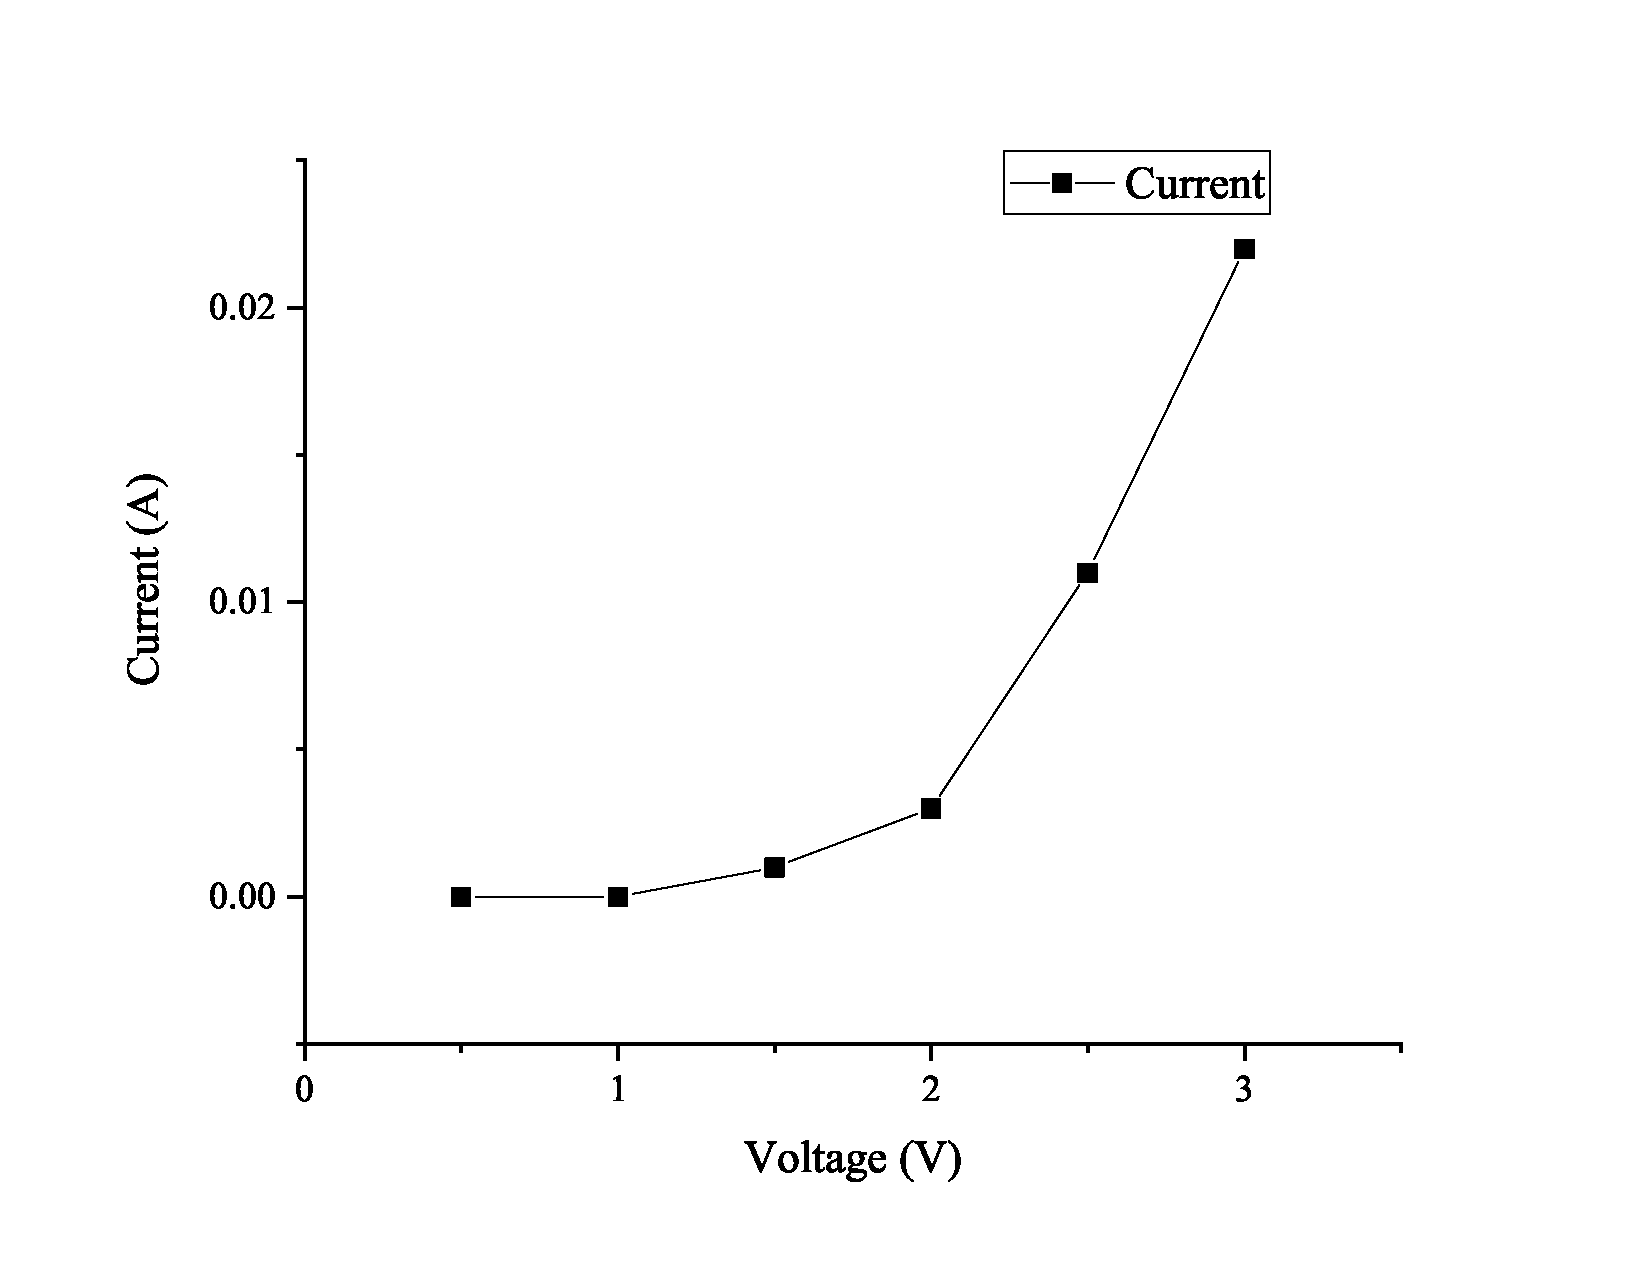
\includegraphics[width=1\linewidth]{7.eps}
		\caption{The voltage-current characteristic curve for LED.}
	\end{figure}
	We can see that the graph is quite in accordance with the expectation of the theorectical model, and the trun-on voltage is about 1.6V as expected in the last part of the section 1.2.
	\section{Conclusions and Discussion}
	In this experiment, we managed to verify Kirchhoff's current and voltage laws and the Ohm's law by measuring the resistances, plotting a fitting curve, and sketching a voltage-current characteristic curve for semiconductors like LED. The data and the corresponding graphs are applicable in accordance with our expectation, so the experiment is generally successful.
	
	The source of uncertainty comes from the hand operation on the multimeter and the resistance of conducting wires, even though they are relatively neglictable. Besides, they are very hot shortly after conducting, so it is dangerous to directly touch them with our hand.
	
	Last but not least, we learned the usage of the multimeter and voltage source and began designing circuits for certain purpose, which helps us further develop knowledge of electric circuits.
	\vspace{15cm}
	\section*{Data Sheet}
\end{document}